\documentclass[../../../interview-questions.tex]{subfiles}

\begin{document}

\section{Java}

\subsection{Java问题}

Java获取Class的三种方法:

\begin{lstlisting}[language=Java]
Class<?> class = ClassName.class;
Class<?> class = Class.forName("类名全路径");
Class<?> class = object.getClass();
\end{lstlisting}

\paragraph{Java的BigDecimal如何解决浮点数精度问题}

BigDecimal的解决方案就是,不使用二进制,而是使用十进制(BigInteger)+小数点位置(scale)来表示小数.当使用BigDecimal来进行运算时,也就可以分解成两部分,BigInteger间的运算,以及小数点位置scale的更新.BigInteger可以表示任意精度的整数。当你使用long类型进行运算,可能会产生溢出时就要考虑使用BigInteger了。BigDecimal就使用了BigInteger作为backend。那么BigInteger是如何做到可以表示任意精度的整数的?答案是使用数组来表示.

\begin{lstlisting}[language=Java]
public static void main(String[] args)  {
    byte[] mag = {
            2, 1 // 10 00000001 == 513
    };
    System.out.println(new BigInteger(mag));
}
\end{lstlisting}

如何避免精度问题?在使用的时候,有两种方法:

使用new BigDecimal(String);
使用BigDecimal.valuOf(Double);

即先转成字符串再转成BigDecimal。BigDecimal.valueOf(double)其实就等同于new BigDecimal(String)。

\paragraph{Java栈溢出(StackOverflowError)}

递归调用方法如果递归的深度过深,就会出现栈溢出(StackOverflowError)异常。如果这个区域允许动态扩展,但是无法申请到足够的内存,也会出现栈溢出。调整栈溢出的大小Xss(Stack Size)。最简单的方法就是细致的检查stack trace,找出行号的重复模式。这些重复的行号代表了被递归调用的代码。确认递归实现没有问题,你可以通过-Xss参数增加栈的大小,这个参数可以在项目配置或命令行指定。

\paragraph{Java汇编}

查看汇编代码前,编译成class文件:

\begin{lstlisting}[language=Bash]
javac Bar.java
\end{lstlisting}


如下命令打印汇编指令:

\begin{lstlisting}[language=Bash]
java -Xcomp -XX:+UnlockDiagnosticVMOptions -XX:+PrintAssembly -Xcomp -XX:CompileCommand=dontinline,*Bar.sum -XX:CompileCommand=compileonly,*Bar.sum Bar
\end{lstlisting}

汇编示例如下:
 
\begin{lstlisting}[language=Bash]
Loaded disassembler from /Library/Java/JavaVirtualMachines/jdk1.8.0_112.jdk/Contents/Home/jre/lib/hsdis-amd64.dylib
Decoding compiled method 0x00000001086484d0:
Code:
[Disassembling for mach='i386:x86-64']
[Entry Point]
[Constants]
  # {method} {0x0000000107847230} 'sum' '()V' in 'Bar'
  #           [sp+0x40]  (sp of caller)
  0x0000000108648620: mov    0x8(%rsi),%r10d
  0x0000000108648624: shl    $0x3,%r10
  0x0000000108648628: cmp    %rax,%r10
  0x000000010864862b: jne    0x0000000108584e20  ;   {runtime_call}
  0x0000000108648631: data32 data32 nopw 0x0(%rax,%rax,1)
  0x000000010864863c: data32 data32 xchg %ax,%ax
\end{lstlisting}

\paragraph{负载均衡(Load Balance)的原理}

从应用场景上来说,常见的负载均衡模型有全局负载均衡和集群内负载均衡,从产品形态角度来说,又可以分为硬件负载均衡和软件负载均衡。全局负载均衡一般通过DNS实现,通过将一个域名解析到不同VIP,来实现不同的region调度能力;硬件负载均衡器常见的有F5、A10、Array,它们的优缺点都比较明显,优点是功能强大,有专门的售后服务团队,性能比较好,缺点是缺少定制的灵活性,维护成本较高;现在的互联网更多的思路是通过软件负载均衡来实现,这样可以满足各种定制化需求,常见的软件负载均衡有 LVS、Nginx、Haproxy。系统的扩展可分为纵向(垂直)扩展和横向(水平)扩展。纵向扩展,是从单机的角度通过增加硬件处理能力,比如CPU处理能力,内存容量,磁盘等方面,实现服务器处理能力的提升,不能满足大型分布式系统(网站),大流量,高并发,海量数据的问题。因此需要采用横向扩展的方式,通过添加机器来满足大型网站服务的处理能力。

\subparagraph{轮询调度}

轮询调度(Round Robin Scheduling)算法\footnote{\url{https://blog.csdn.net/u012891504/article/details/53434704}}就是以轮询的方式依次将请求调度到不同的服务器,即每次调度执行i = (i + 1) mod n,并选出第i台服务器。算法的优点是其简洁性,它无需记录当前所有连接的状态,所以它是一种无状态调度。在实际实现过程中,一般会为每台服务器设定一个权重值,这就是权重轮询调度算法。

\subparagraph{IP负载均衡}

在网络层通过修改请求目标地址进行负载均衡。用户请求数据包,到达负载均衡服务器后,负载均衡服务器在操作系统内核进程获取网络数据包,根据负载均衡算法得到一台真实服务器地址,然后将请求目的地址修改为,获得的真实ip地址,不需要经过用户进程处理。

\begin{figure}[htpb]
	\centering
	\caption{IP负载均衡}
	\label{fig:iploadbalance}
	\begin{tikzpicture}
		\node (user) [rectangle, draw=blue!50, fill=blue!20] {用户};
	    \node (loadbalancer) [rectangle, draw=blue!50, fill=blue!20] {负载均衡服务器};
	    \node (appserver1) [circle, right=of loadbalancer, draw=red!50, fill=red!20] {192.168.1.11};
	    \node (appserver2) [circle, left=of loadbalancer, draw=red!50, fill=red!20] {192.168.1.12};
	    \draw[->, bend right] (loadbalancer) edge (appserver1);
	    \draw[<-] (loadbalancer) -- (appserver1);
	\end{tikzpicture}
\end{figure}



\paragraph{Long比较}

如果Long的值在[-127,128]之间,用“==”判断是否相等是没问题的,如果不在这个区间,是不能用“==”的,原因如下源码解释:

\begin{lstlisting}[language=Java]
public static Long valueOf(long l) {
    final int offset = 128;
    if (l >= -128 && l <= 127) { // will cache
        return LongCache.cache[(int)l + offset];
    }
    return new Long(l);
}
\end{lstlisting}

如果不在[-127,128]之间,则会new一个新对象,自然“==”两个不同的对象,其结果必然是false了。Long中有一个静态的内部类LongCache,专门用于缓存-128至127之间的值,一共256个元素。
如果仅仅是缓存下来而不去使用那么就没有任何意义。valueOf(long l)就是使缓存派上用场的方法,它会判断传入的参数是否在-128-127之间,如果是则直接从缓存中返回对应的引用,否则新创建一个Long的实例。JVM具有跨平台性因此long在32位和64位机下基本数据类型占字节数是一致的,不过要注意long在32位机器上的赋值操作不是原子性的。

\begin{lstlisting}[language=Java]
Long l1 = new Long(100);
Long l2 = new Long(200);
System.out.println(l1.longValue()<l2.longValue());
\end{lstlisting}

缓存的目的主要是节省内存、提高性能、避免创建新的装箱对象,其他考量需要问设计Java规范那几爷子了\footnote{\url{https://stackoverflow.com/questions/55897693/why-java-integerlong-cached-128-127?noredirect=1\#comment9845168255897693}}。

\paragraph{WeakHashMap和HashMap的区别}

“引用”,在Java中指的是一个对象对另一对象的使用(指向)。WeakHashMap中的键的类型是WeakReference,在Java中还有另外两种引用:强引用(Strong Reference)、软引用(Soft Reference)。被SoftReference指向的对象可能会被垃圾收集器回收,但是只有在JVM内存不够的情况下才会回收,当一个对象仅仅被WeakReference引用时,在下个垃圾收集周期时候该对象就会被回收。有的时候HashMap中的对象不再使用,此时需要手动删除元素,才能够释放内存,但是有时候找出来不使用的元素比较繁琐,此时就可以使用WeakHashMap来自动释放内存,详细可以参考\footnote{\url{https://www.ibm.com/developerworks/cn/java/j-jtp11225/index.html}}。


\paragraph{Java 8 Stream效率}

对于简单操作,比如最简单的遍历,Stream串行API性能明显差于显示迭代,但并行的Stream API能够发挥多核特性。
对于复杂操作,Stream串行API性能可以和手动实现的效果匹敌,在并行执行时Stream API效果远超手动实现。
所以,如果出于性能考虑,对于简单操作推荐使用外部迭代手动实现,对于复杂操作,推荐使用Stream API,在多核情况下,推荐使用并行Stream API来发挥多核优势,单核情况下不建议使用并行Stream API。如果出于代码简洁性考虑,使用Stream API能够写出更短的代码。即使是从性能方面说,尽可能的使用Stream API也另外一个优势,那就是只要Java Stream类库做了升级优化,代码不用做任何修改就能享受到升级带来的好处。

\paragraph{泛型(Generic)-参数化类型}

Java语言引入泛型的好处是安全简单,可以在在编译的时候检查类型安全,避免由于类型转换失败程序在运行时抛出异常。同时,泛型还可以消除代码中许多的强制类型转换(强制类型转换很消耗性能),带来了性能上的收益,并且所有的强制转换都是自动和隐式的,泛型也提高代码的重用率。

\paragraph{类型擦除(Type Erasure)}

泛型的实现思路有两种\footnote{\url{https://www.cnblogs.com/fsjohnhuang/p/4288614.html}}:



C++的模板和C\# 就是典型的Code Specialization。由于在程序中出现N种L泛型List则会生成N个Class实例,因此会造成代码膨胀(Code Bloat)。而Java则采用Code Sharing的思路,并通过类型擦除(Type Erasure)来实现。类型擦除的过程大致分为两步:


用如下代码片段来观察类型擦除,在没有类型搽除前:

\begin{lstlisting}[language=Java]
Map<String, String> map = new HashMap<String, String>();
map.put("hello", "你好");
\end{lstlisting}

采用javac编译后,查看泛型擦除后的代码为:

\begin{lstlisting}[language=Java]
HashMap var1 = new HashMap();
var1.put("hello", "你好");
\end{lstlisting}

擦除法所谓的擦除,仅仅是对方法的 Code 属性中的字节码进行擦除,实际上元数据中还是保留了泛型信息,这也是我们能通过反射手段取得参数化类型的根本依据。

\paragraph{获取实际类型}

既然泛型擦除了类型,那么怎么获取到实际到类型呢\footnote{\url{https://blog.csdn.net/hj7jay/article/details/54889717}}?

在Java中,泛型类型虽然被擦除了\footnote{参见:\url{https://segmentfault.com/a/1190000020382440}},但是被擦除的类型信息还是会以某种形式存储下来,并支持在运行时获取。这种形式就是指元素附加的签名信息(Signatures),谷歌是这么定义Signatures:

Signatures encode declarations written in Java programming language that use types outside the type system of the Java Virtual Machine. They support reflection and debugging, as well as compilation when only class files are available.

\paragraph{字符串比较}

String s1 = "Hello World"; String s2 = "Hello World"; a==b的结果是什么? 这包含了内存,String存储方式等诸多知识点。

\begin{lstlisting}[language=Java]
String s1 = "hello,world!";
String s2 = "hello,world!";
System.out.println(s1 == s2); // True
\end{lstlisting}

== 操作符比较的是两个对象的引用是否指向同一内存地址,如果内存地址相同,则返回 true;equals() 比较的只是两个字符串对象的引用指向的内存地址所存储的字面值,而忽略内存地址是否相同。


\paragraph{红黑树(Red–black tree)}

它在1972年由鲁道夫·贝尔发明,被称为"对称二叉B树",它现代的名字源于Leo J. Guibas和Robert Sedgewick于1978年写的一篇论文\footnote{\url{https://zh.wikipedia.org/wiki/红黑树}}。红黑树和AVL树一样都对插入时间、删除时间和查找时间提供了最好可能的最坏情况担保。这不只是使它们在时间敏感的应用,如实时应用(real time application)中有价值,而且使它们有在提供最坏情况担保的其他数据结构中作为基础模板的价值;例如,在计算几何中使用的很多数据结构都可以基于红黑树实现。红黑树是每个节点都带有颜色属性的二叉查找树,颜色为红色或黑色。在二叉查找树强制一般要求以外,对于任何有效的红黑树增加了如下的额外要求:

\begin{enumerate}
\item {节点是红色或黑色。}
\item{根是黑色。}
\item{所有叶子都是黑色(叶子是NIL节点)--"nil叶子"或"空(null)叶子。}
\item{每个红色节点必须有两个黑色的子节点。(从每个叶子到根的所有路径上不能有两个连续的红色节点。)}
\item{从任一节点到其每个叶子的所有简单路径都包含相同数目的黑色节点。}
\end{enumerate}

\paragraph{dispatchServlet怎样分发任务的}


1). 用户发请求-->DispatcherServlet,前端控制器收到请求后自己不进行处理,而是委托给其他的解析器进行处理,作为统一访问点,进行全局的流程控制。

2).DispatcherServlet-->HandlerMapping,HandlerMapping将会把请求映射为HandlerExecutionChain对象(包含一个Handler处理器,多个HandlerInterceptor拦截器)。

3).DispatcherServlet-->HandlerAdapter,HandlerAdapter将会把处理器包装为适配器,从而支持多种类型的处理器。

4).HandlerAdapter-->处理器功能处理方法的调用,HandlerAdapter将会根据适配的结果调用真正的处理器的功能处理方法,完成功能处理,并返回一个ModelAndView对象(包含模型数据,逻辑视图名)

5).ModelAndView的逻辑视图名-->ViewResolver,ViewResoler将把逻辑视图名解析为具体的View。

6).View-->渲染,View会根据传进来的Model模型数据进行渲染,此处的Model实际是一个Map数据结构

7).返回控制权给DispatcherServlet,由DispatcherServlet返回响应给用户。

\paragraph{private修饰的方法可以通过反射访问,那么private的意义是什么}

private是声明方法的允许访问范围,偏向于OOP的设计原则,并不是为了绝对安全而设计。只提供内部类调用的方法有private修饰后,外部类调用时可以更清晰简洁(不会出现许多根本用不到或者完全没必要暴露给外部类的方法)。反射偏重逆向操作,舍弃了部分性能和安全,获取了部分的便捷性和灵活性,需要掌控好平衡。可以理解为private定义了一个规则,但是某些情况下,可以特事特办。可以不遵守规则,但是需要承担一些风险\footnote{\url{https://stackoverflow.com/questions/1239581/why-is-it-allowed-to-access-java-private-fields-via-reflection/1239690\#1239690}}。


\paragraph{Arrays.sort的实现}

在JDK7以前的版本中sort()的实现原理是:基本类型使用优化后的快速排序,其他类型使用优化后的归并排序,jdk7以后修改了排序策略:如果JVM启动参数配置了-Djava.util.Arrays.useLegacyMergeSort=true那么就会执行上面所说的排序策略(优化的归并排序),否则将会执行TimSort排序\footnote{\url{https://www.jianshu.com/p/d7ba7d919b80}}(此处存疑)。

\paragraph{TreeMap 和 LinkedHashMap 是如何保证它的顺序的}

TreeMap 是通过实现 SortMap 接口,能够把它保存的键值对根据 key 排序,基于红黑树,从而保证 TreeMap 中所有键值对处于有序状态。LinkedHashMap 则是通过插入排序和访问排序(改变排序把访问过的放到底部)让键值有序。

\paragraph{什么时候使用CopyOnArrayList}

CopyOnWriteArrayList这是一个ArrayList的线程安全的变体,其原理大概可以通俗的理解为:初始化的时候只有一个容器,很常一段时间,这个容器数据、数量等没有发生变化的时候,大家(多个线程),都是读取(假设这段时间里只发生读取的操作)同一个容器中的数据,所以这样大家读到的数据都是唯一、一致、安全的,但是后来有人往里面增加了一个数据,这个时候CopyOnWriteArrayList底层实现添加的原理是先copy出一个容器(可以简称副本),再往新的容器里添加这个新的数据,最后把新的容器的引用地址赋值给了之前那个旧的的容器地址,但是在添加这个数据的期间,其他线程如果要去读取数据,仍然是读取到旧的容器里的数据。CopyOnWriteArrayList适合使用在读操作远远大于写操作的场景里,比如缓存。

\paragraph{wait和sleep区别}

sleep是线程类(Thread)的方法,sleep不会交出任何已获得的对象锁.wait是Object类的方法,wait会交出调用wait对象的对象锁。而且wait存在notify方法来唤醒调用wait的线程,这个是sleep没有的。

\paragraph{常见序列化协议及其优缺点}

常见序列化协议有COM、CORBA、XML、JSON、Protobuf、Thrift和Avro\footnote{\url{http://www.dongcoder.com/detail-1031666.html}}。

\paragraph{Protobuf}protobuf(Google Protocol Buffers)
Google提供一个具有高效的协议数据交换格式工具库(类似Json)。
但相比于Json,Protobuf有更高的转化效率,时间效率和空间效率都是JSON的3-5倍。优点是性能好效率高、有代码生成机制、支持向前和向后兼容、支持多种变成语言。缺点是可读性较差、缺少自描述、通用型较差,多平台项目中,可能会涉及到改造和适配工作。JSON使用广泛,开发效率高,性能相对较低,维护成本较高。

\paragraph{Thrift}

\begin{enumerate}
\item {序列化和RPC支持一站式解决,比pb更方便}
\item{跨语言,IDL接口定义语言,自动生成多语言文件}
\item{省流量,体积较小}
\item{包含完整的客户端/服务端堆栈,可快速实现RPC}
\item{为服务端提供了多种工作模式,如线程池模型、非阻塞模型}
\end{enumerate}


\paragraph{http请求报文结构和内容}

HTTP报文结构分为起始行,请求头,请求体。起始行由方法、、URL、HTTP版本组成,以空格分开。请求头和请求体以空行分开。


\paragraph{List、Map、Set的区别与联系}

List和Set都实现了collection接口\footnote{https://www.jianshu.com/p/46a6b4c6693f}。

\begin{figure}[htbp]
	\centering
	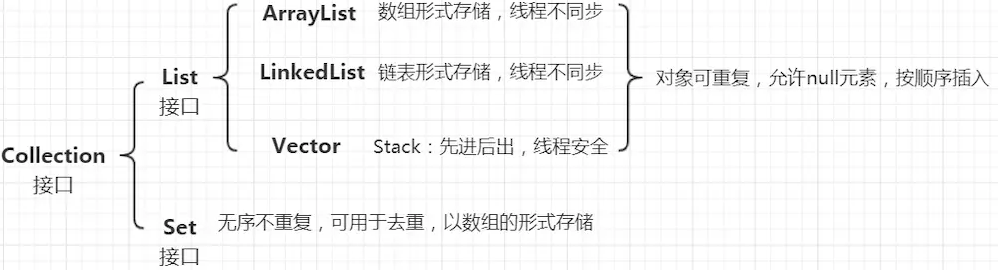
\includegraphics[scale=0.4]{collection.png}
	\caption{List和Set}
	\label{fig:collection}
\end{figure}

\paragraph{什么时候使用LinkedHashMap、ConcurrentHashMap、WeakHashMap}

\paragraph{Java抽象类与接口的区别}

Java在类的继承上并没有多继承。抽象类属于类,所以可以被继承。但子类只能继承一个父类。Java为了实现多继承,使用了接口。一个类可以实现多个接口。如果你往抽象类中添加新的方法,你可以给它提供默认的实现。因此你不需要改变你现在的代码。 如果你往接口中添加方法,那么你必须改变实现该接口的类。

\paragraph{类加载机制和步骤}

 类从被加载到虚拟机内存中开始,到卸载出内存为止,它的整个生命周期包括:加载(Loading)、验证(Verification)、准备(Preparation)、解析(Resolution)、初始化(Initialization)、使用(Using)和卸载(Unloading)七个阶段。其中验证(Verification)、准备(Preparation)、解析(Resolution)3个部分统称为连接(Linking).

\subparagraph{加载}通过一个类的全限定名来获取定义此类的二进制字节流。
将这个字节流所代表的静态存储结构转化为方法区的运行时数据结构。
在内存中生成一个代表这个类的java.lang.Class对象,作为方法区这个类的各种数据的访问入口。

\subparagraph{验证}验证是连接阶段的第一步,这一阶段的目的是为了确保Class文件的字节流中包含的信息符合当前虚拟机的要求,并且不会危害虚拟机自身的安全。

\subparagraph{准备}准备阶段是正式为类变量分配内存并设置类变量初始值得阶段,这些变量所使用的内存都讲在方法区中进行分配。这时候进行内存分配的仅包括类变量(被static修饰的变量),而不包括实例变量,实例变量将会在对象实例化时随着对象一起分配在Java堆中。

\paragraph{哪些集合类是线程安全的}

Vector/HashTable/ConcurrentHashMap/Stack.


\paragraph{为什么集合类Collection不实现Cloneable和Serializable接口}

Collection接口指定一组称为元素的对象。元素如何被组织取决于具体实现。例如,一些LIST实现允许重复的元素,而SET不允许。Collection是一种抽象表示,而克隆和序列化重在执行,应该是在Collection具体实现子类中根据具体元素组织情况来实现。因此,强制在所有实现都要有克隆和序列化是不够灵活的,具有限制性。


\paragraph{HashMap 、HashTable、TreeMap、LinkedHashMap、ConcurrentHashMap 、WeakHashMap}

LinkedHashMap是HashMap的一個子類,如果需要輸出的順序和輸入相同,那麼用LinkedHashMap可以實現、它還可以按讀取順序來排列。WeakHashMap中key採用的是“弱引用”的方式,只要WeakHashMap中的key不再被外部引用,它就可以被垃圾回收器回收。而HashMap中key採用的是“強引用的方式”,當HashMap中的key沒有被外部引用時,只有在這個key從HashMap中刪除後,才可以被垃圾回收器回收。在JDK1.8中有了一些变化,当链表的存储的数据个数大于等于8的时候,不再采用链表存储,而采用了红黑树存储结构。两个线程同时操作时同时遇到HashMap需要扩容,且映射到相同的地址(key计算得到的HashCode相同),此时在扩容时可能发生一种情况, 两个线程同时对HashMap进行扩容,扩容时做第一次循环时一个线程阻塞,另一个完成扩容,前一个继续,那么就可能发生链表数据的相互指向问题, 造成get数据时遍历的死循环.JDK1.8 中通过测试发现依然存在JDK1.7中的数据丢失情况\footnote{\url{http://linfenliang.com/hashmap/2017/08/04/HashMapInJDK-6-7-8-Differ/}}.

\begin{table}[htbp]
	\caption{Map时间复杂度}
	\label{table:mapo1}
	\begin{center}
		\begin{tabular}{|c|c|p{5cm}|}
			\hline
			\multirow{1}{*}{Type}
			& \multicolumn{1}{c|}{获取} 
			& \multicolumn{1}{c|}{查找}\\			
			\cline{1-3}
			ArrayList &  O(1)  &  O(1) \\
			\hline
			HashMap &  O(N/BucketSize)  & O(N/BucketSize)  \\
			\hline							
		\end{tabular}	
	\end{center}
\end{table}



\paragraph{HashMap里的hashcode方法和equal方法什么时候需要重写?如果不重写会有什么后果?}

当在HashMap里以非基本类型作为key时,或者是比较非基本类型时。如果用非基本类型对象作为HashMap的key时不重写的话,会无法正常获取到对应的值,无法正确的按照预期写入对象和获取对象\footnote{参考:\url{https://www.journaldev.com/21095/java-equals-hashcode}}。

\paragraph{hashcode实现原理}


hashcode Java虚拟机实现是C++实现的,代码在synchronizer.cpp文件的方法get\_next\_hash\footnote{\url{https://hg.openjdk.java.net/jdk8/jdk8/hotspot/file/tip/src/share/vm/runtime/synchronizer.cpp}}中(没看懂)。hashcode String的实现如下代码片段所示:

\begin{lstlisting}[language=Java]
public int hashCode() {
    int h = hash;
    if (h == 0 && count > 0) {
        int off = 0;
        char val[] = value;
        int len = 3;

        for (int i = 0; i < 3; i++) {
            h = 31*h + val[off++];
        }
        hash = h;
    }
    return h;
}
\end{lstlisting}



它实际执行的运算是:$s[0]*31^{(n-1)} + s[1]*31^{(n-2)} + ... + s[n-1]$\footnote{\url{https://stackoverflow.com/questions/299304/why-does-javas-hashcode-in-string-use-31-as-a-multiplier}}。选择31作为乘子,hash可以直接位移运算,提高性能,更加重要的是采用31作为乘子,hash分布均匀,太小的乘子分布不均匀很容易冲突,太大的乘子非常容易溢出整型范围,信息容易丢失\footnote{\url{https://segmentfault.com/a/1190000010799123}}(溢出后也没有明显的hash冲突提高现象)。

\paragraph{HashMap是如何定位元素的}

在每个数组元素上都一个链表结构,当数据被Hash后,得到数组下标,把数据放在对应下标元素的链表上。例如程序执行下面代码:

\begin{lstlisting}[language=Java]
map.put("dolphin","小强");
\end{lstlisting}

系统将调用”dolphin”这个key的hashCode()方法得到其hashCode 值(该方法适用于每个Java对象),然后再通过Hash算法的后两步运算来定位该键值对的存储位置,有时两个key会定位到相同的位置,表示发生了Hash碰撞。HashMap存取时,都需要计算当前key应该对应Entry[]数组哪个元素,即计算数组下标;算法如下:

\begin{lstlisting}[language=Java]
/**
* Returns index for hash code h.
*/
static int indexFor(int h, int length) {
	return h & (length-1);
}
\end{lstlisting}

按位取并,作用上相当于取模mod或者取余\%。这意味着数组下标相同,并不表示hashCode相同。


\paragraph{HashMap put()元素产生冲突,为什么用LinkedList(拉链法)而不用ArrayList解决,产生冲突时key值不等,新元素怎样加入链表,为什么这么设计}

HashMap key冲突属于特殊情况,不是常规情况,ArrayList的初始长度是10,如果使用ArrayList,绝大多数情况下ArrayList只有一个元素,会造成资源的浪费。从ArrayList中删除最后一个元素代价很小,但是删除第一个元素时,需要移动之后的所有元素,代价很大。LinkedList插入和删除复杂度都是O(1)\footnote{\url{https://stackoverflow.com/questions/30414427/why-linkedlist-in-hashmapwhy-not-other-implementation-of-list}},更严谨的说法是从尾部插入是O(1),从指定位置插入是O(n),因为链表是顺序访问,找到元素的复杂度是O(n)。

\paragraph{Iterator和Enumeration区别}

Enumeration只有2个函数接口。通过Enumeration,我们只能读取集合的数据,而不能对数据进行修改.Iteration只有3个函数的接口。Iteration除了能读取集合的数据之外,也能对数据进行删除.Iterator支持Fail-Fast机制,当一个线程在遍历时,不允许另外一个线程对数据进行修改(除非调用实现了Iterator的Remove方法)。因此Iterator被认为是安全可靠的遍历方式\footnote{\url{https://www.cnblogs.com/yixianyixian/p/7687492.html}}.


\paragraph{ArrayList和LinkedList底层实现有什么差别?它们各自适用于哪些场合?}

ArrayList 是基于动态数组数据结构的实现,访问元素速度优于 LinkedList。LinkedList 是基于链表数据结构的实现,占用的内存空间比较大,但在批量插入或删除数据时优于 ArrayList。注意这里的插入要区分插入头尾。数组在内存中是顺序存储,在内存中是占用一块块连续的内存空间,数组元素之间紧密排列,即不能打乱元素排列顺序,也不能跳过某个存储单元进行存储。尾部插入:尾部插入最简单,直接在尾部追加。中间插入:稍许复杂,需要把插入位置的元素及后面的元素向后移动,为插入元素腾出空间。超范围插入:因数组的容量在创建时就确定的,如果需要超范围插入,就涉及数给扩容,通常是创建一个新数给,为旧数组的 2 倍,在把旧数组中的元素全部复制到新数组。数组根据元素下标删除,实际是把要删除的元素的后面元素向前挪动 1 位,覆盖要删除的元素。若没有顺序要求,可将最后一个元素赋值给要删除的元素的位置,这就无须进行大量的元素移动。链表(Linked list):是一种在物理上 非连续、非顺序的数据结构,由若干节点(node)所组成。链表在内存中的存储方式是 随机存储,这样可以有效地利用零散的碎片空间。LinkedList 是链表的操作

get() 获取第几个元素,依次遍历,复杂度O(n)

add(E) 添加到末尾,复杂度O(1)

add(index, E) 添加第几个元素后,需要先查找到第几个元素,直接指针指向操作,复杂度O(n)

remove()删除元素,直接指针指向操作,复杂度O(1)

对于快速访问对象的需求,使用 ArrayList 实现执行效率上会比较好。需要频繁向集合中插入和删除元素时,使用 LinkedList 类比 ArrayList 类效果高。

\paragraph{Java中==和equals有什么区别}

原始数据类型(byte,short,char,int,long,float,double,boolean),他们之间的比较使用(==),比较的是他们的值。引用数据类型用(==)进行比较,比较的是他们在内存中的存放地址。equals如果没有自己的实现,原始类型默认比较其值,引用类型默认比较内存地址。

\paragraph{CompletableFuture,这个是JDK1.8里的新特性,通过它怎么实现多线程并发控制?}


\paragraph{JDK、JRE和JVM三者之间关系}

JDK(Java Development Kit)是针对Java开发员的产品,是整个Java的核心,包括了Java运行环境JRE、Java工具和Java基础类库。Java Runtime Environment(JRE)是运行JAVA程序所必须的环境的集合,包含JVM标准实现及Java核心类库。JVM是Java Virtual Machine(Java虚拟机)的缩写,是整个java实现跨平台的最核心的部分,能够运行以Java语言写作的软件程序。
JDK是java开发工具包,在其安装目录下面有六个文件夹、一些描述文件、一个src压缩文件。bin、include、lib、 jre这四个文件夹起作用,demo、sample是一些例子。可以看出来JDK包含JRE,而JRE包含JVM。

\begin{enumerate}
	\item{bin:最主要的是编译器(javac.exe)}
	\item{include:java和JVM交互用的头文件}
	\item{lib:类库}
	\item{jre:java运行环境(注意:这里的bin、lib文件夹和jre里的bin、lib是不同的)}
\end{enumerate}

总的来说JDK是用于Java程序的开发,而jre则是只能运行class而没有编译的功能。JDK是提供给Java开发人员使用的,其中包含了java的开发工具,也包括了JRE。所以安装了JDK,就不用在单独安装JRE了。其中的开发工具包括编译工具(javac.exe)打包工具(jar.exe)等。JRE是指java运行环境。光有JVM还不能成class的执行,因为在解释class的时候JVM需要调用解释所需要的类库lib。在JDK的安装目录里你可以找到jre目录,里面有两个文件夹bin和lib,在这里可以认为bin里的就是jvm,lib中则是jvm工作所需要的类库,而jvm和lib和起来就称为jre。所以,在你写完java程序编译成.class之后,你可以把这个.class文件和jre一起打包发给朋友,这样你的朋友就可以运行你写程序了。包括Java虚拟机(JVM Java Virtual Machine)和Java程序所需的核心类库等,如果想要运行一个开发好的Java程序,计算机中只需要安装JRE即可。



\paragraph{Lucene全文搜索的原理}

Lucene全文搜索基于倒排索引(Reverted Index),主要分为2方面,建立索引和检索。建立索引的流程如下:


检索的流程如下:

\paragraph{如何设计存储海量数据的存储系统}

\paragraph{为什么PostgreSQL最大的单表只能是32TB}

在PostgreSQL中,一张表对应多个数据文件。
数据文件中存储的是page,每一个page都有一个单独的编号,因为pg寻址空间采用的是32位,也就是$2^{32}=4294967296$,也就是一组数据文件中最多存放这些page。
按照默认的block\_size设置为8K,可以计算出来一组数据文件最大的大小是32TB。


$2^{32} \times 8 \div 1024 \div 1024 \div 1024 = 32TB$


\subsection{多线程问题}

\paragraph{怎么检测一个线程是否持有对象监视器}

Thread类提供了一个holdsLock(Object obj)方法,当且仅当对象obj的监视器被某条线程持有的时候才会返回true,注意这是一个static方法,这意味着”某条线程”指的是当前线程。

\paragraph{Runnable和Callable的区别}

Runnable接口中的run()方法的返回值是void,它做的事情只是纯粹地去执行run()方法中的代码而已;Callable接口中的call()方法是有返回值的,是一个泛型,和Future、FutureTask配合可以用来获取异步执行的结果。
这其实是很有用的一个特性,因为多线程相比单线程更难、更复杂的一个重要原因就是因为多线程充满着未知性,某条线程是否执行了?某条线程执行了多久?某条线程执行的时候我们期望的数据是否已经赋值完毕?无法得知,我们能做的只是等待这条多线程的任务执行完毕而已。而Callable+Future/FutureTask却可以方便获取多线程运行的结果,可以在等待时间太长没获取到需要的数据的情况下取消该线程的任务.

\subsection{Java类文件结构}

Java类文件结构如下表\footnote{参考:\url{https://en.wikipedia.org/wiki/Java_class_file}}所示:

\begin{table}[htbp]
	\caption{Java类文件结构}
	\label{table:mapo2}
	\begin{center}
		\begin{tabular}{cp{5cm}c}
			\hline
			\multirow{1}{*}{占用大小}
			& \multicolumn{1}{c}{字段描述} 
			& \multicolumn{1}{c}{数量}\\			
			\cline{1-3}
			4bit &  magic:魔数,用于标识文件类型,对于java来说是0xCAFEBABE  &  1 \\
			\hline
			2bit &  minor\_version:次版本号 & 1 \\
			\hline
			2bit &  major\_version:主版本号 & 1 \\
			\hline							
		\end{tabular}	
	\end{center}
\end{table}

使用javap输出常量表:

\begin{figure}[htbp]
	\centering
	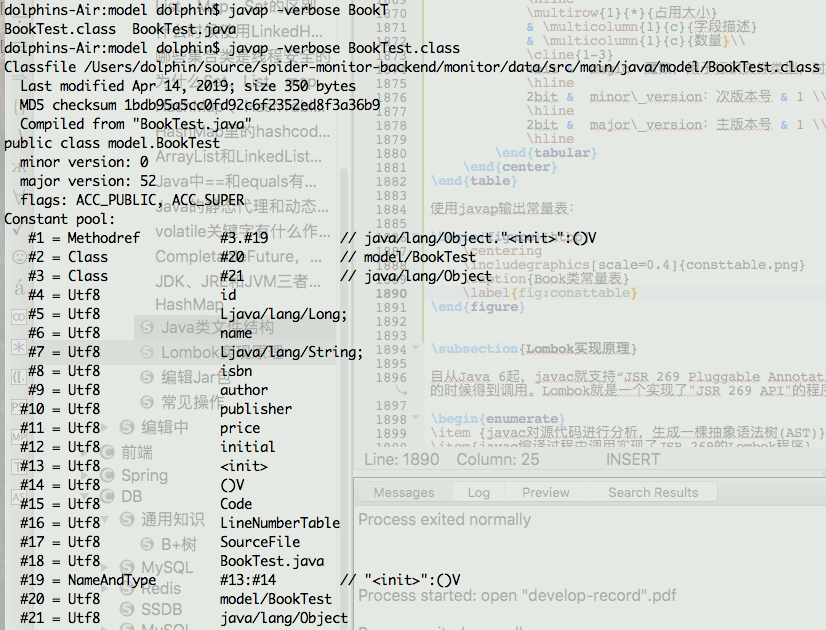
\includegraphics[scale=0.5]{consttable.png}
	\caption{Book类常量表}
	\label{fig:consttable}
\end{figure}


\subsection{Lombok实现原理}

自从Java 6起,javac就支持“JSR 269 Pluggable Annotation Processing API”规范,只要程序实现了该API,就能在javac运行的时候得到调用。Lombok就是一个实现了"JSR 269 API"的程序。在使用javac的过程中,它产生作用的具体流程如下:

\begin{enumerate}
\item {javac对源代码进行分析,生成一棵抽象语法树(AST)}
\item{javac编译过程中调用实现了JSR 269的Lombok程序}
\item{此时Lombok就对第一步骤得到的AST进行处理,找到Lombok注解所在类对应的语法树(AST),然后修改该语法树(AST),增加Lombok注解定义的相应树节点}
\item{javac使用修改后的抽象语法树(AST)生成字节码文件}
\end{enumerate}

\section{框架(Framework)}

\subsection{Spring MVC还是WebFlux}

\subsection{Sring Bean创建过程}

获取参数 name 对应的真正的 beanName
检查缓存或者实例工厂中是否有对应的单例,若存在则进行实例化并返回对象,否则继续往下执行
执行 prototype 类型依赖检查,防止循环依赖
如果当前 beanFactory 中不存在需要的 bean,则尝试从 parentBeanFactory 中获取
将之前解析过程返得到的 GenericBeanDefinition 对象合并为 RootBeanDefinition 对象,便于后续处理
如果存在依赖的 bean,则递归加载依赖的 bean
依据当前 bean 的作用域对 bean 进行实例化
如果对返回 bean 类型有要求,则进行检查,按需做类型转换
返回 bean 实例


Sring Bean创建过程简单分为7个步骤。

\begin{enumerate}
\item{获取beanName}
\item{实例化bean}
\item{单例(Singleton)依赖处理}
\item{属性填充}
\item{原型(Prototype)依赖检查}
\item{注册DisposableBean}
\end{enumerate}


\begin{enumerate}
\item{如果是单例则需要首先清除缓存} 
\item{实例化bean,将BeanDefinition转换为BeanWrapper}
转换是一个复杂的过程,但是我们可以尝试概括大致的功能:

如果存在工厂方法则使用工厂方法进行初始化
一个类有多个构造函数,每个构造函数都有不同的参数,所以需要根据参数锁定构造函数并进行初始化
如果既不存在工厂方法也不存在带有参数的构造函数,则使用默认的构造函数进行 bean 的实例化.首先就是创建一个bean的实例且封装到BeanWrapper中,在这里bean已经实例化了。具体的实现方法是在SimpleInstantiationStrategy类的方法instantiate中。

\item{MergedBeanDefinitionPostProcessor的应用}
bean合并后的处理,Autowired注解正是通过此方法实现诸如类型的预解析。

\item{依赖处理}
在Spring中会有循环依赖的情况,例如,当A中含有B的属性,而B中又含有A的属性时就会构成一个循环依赖,此时如果A和B都是单例,那么在Spring中的处理方式就是当创建B的时候,涉及自动注入A的步骤时,并不是直接去再次创建A,而是通过放入缓存中的ObjectFactory来创建实例,这样就解决了循环依赖的问题。

\item{属性填充。将所有属性填充至bean的实例中}findAutowiringMetadata方法能拿到使用了特定注解的属性(Field)、方法(Method)及依赖的关系保存到checkedElements集合<Set>里,然后再执行自己的inject方法。设置值的关键代码,实质就是通过JDK的反射特性:


\begin{lstlisting}[language=Java]
Field field = (Field) this.member;
ReflectionUtils.makeAccessible(field);
field.set(target, getResourceToInject(target, requestingBeanName));
\end{lstlisting}



\item{循环依赖检查}
Spring 中解决循环依赖只对单例有效,而对于 prototype 的 bean,Spring 没有好的解决办法,唯一要做的就是抛出异常。在这个步骤里面会检测已经加载的 bean 是否已经出现了依赖循环,并判断是否需要抛出异常。

\item{注册DisposableBean}
如果配置了destroy-method,这里需要注册以便于在销毁时候调用。

\item{完成创建并返回}

\end{enumerate}

\section{多线程(Multi-Thread)}

\subsection{线程同步以及线程调度相关的方法}

\begin{enumerate}
\item {wait():使一个线程处于等待(阻塞)状态,并且释放所持有的对象的锁;}
\item{sleep():使一个正在运行的线程处于睡眠状态,是一个静态方法,调用此方法要处理InterruptedException异常;}
\item{notify():唤醒一个处于等待状态的线程,当然在调用此方法的时候,并不能确切的唤醒某一个等待状态的线程,而是由JVM确定唤醒哪个线程,而且与优先级无关;}
\item{notityAll():唤醒所有处于等待状态的线程,该方法并不是将对象的锁给所有线程,而是让它们竞争,只有获得锁的线程才能进入就绪状态;}
\end{enumerate}

\subsubsection{Moniter的实现原理}

无论是同步方法还是同步代码块,无论是ACC\_SYNCHRONIZED还是monitorenter、monitorexit都是基于Monitor实现的,什么是Monitor?

\begin{quotation}
管程 (英语:Monitors,也称为监视器) 是一种程序结构,结构内的多个子程序(对象或模块)形成的多个工作线程互斥访问共享资源。这些共享资源一般是硬件设备或一群变量。管程实现了在一个时间点,最多只有一个线程在执行管程的某个子程序。与那些通过修改数据结构实现互斥访问的并发程序设计相比,管程实现很大程度上简化了程序设计。 管程提供了一种机制,线程可以临时放弃互斥访问,等待某些条件得到满足后,重新获得执行权恢复它的互斥访问。
\end{quotation}

在Java虚拟机(HotSpot)中,Monitor是基于C++实现的,由ObjectMonitor\footnote{\url{https://github.com/openjdk-mirror/jdk7u-hotspot/blob/50bdefc3afe944ca74c3093e7448d6b889cd20d1/src/share/vm/runtime/objectMonitor.cpp}}实现的,其主要数据结构如下:

\begin{lstlisting}[language=C++]
ObjectMonitor::ObjectMonitor() {  
  _header       = NULL;  
  _count       = 0;  
  _waiters      = 0,  
  _recursions   = 0;       //线程的重入次数
  _object       = NULL;  
  _owner        = NULL;    //标识拥有该monitor的线程
  //等待线程组成的双向循环链表,\_WaitSet是第一个节点
  _WaitSet      = NULL;    
  _WaitSetLock  = 0 ;  
  _Responsible  = NULL ;  
  _succ         = NULL ;  
  _cxq          = NULL ;    //多线程竞争锁进入时的单向链表
  FreeNext      = NULL ;
  //\_owner从该双向循环链表中唤醒线程结点,\_EntryList是第一个节点  
  _EntryList    = NULL ;    
  _SpinFreq     = 0 ;  
  _SpinClock    = 0 ;  
  OwnerIsThread = 0 ;  
}
\end{lstlisting}

\subsubsection{Synchronized优化}

早期,Synchronized属于重量级锁(Heavyweight Lock),效率低下,因为监视器锁(monitor)是依赖于底层的操作系统的Mutex Lock来实现的,而操作系统实现线程之间的切换时需要从用户态(User Model)转换到核心态(Kernel Model)\footnote{从用户态到内核态切换过程中,Linux主要做的事:

1:读取tr寄存器,访问TSS段

2:从TSS段中的sp0获取进程内核栈的栈顶指针

3:  由控制单元在内核栈中保存当前eflags,cs,ss,eip,esp寄存器的值。

4:由SAVE\_ALL保存其寄存器的值到内核栈

5:把内核代码选择符写入CS寄存器,内核栈指针写入ESP寄存器,把内核入口点的线性地址写入EIP寄存器},这个状态之间的转换需要相对比较长的时间\footnote{\url{https://www.cnblogs.com/justcxtoworld/p/3155741.html}},时间成本相对较高,这也是为什么早期的synchronized效率低的原因。庆幸的是在Java 6之后Java官方对从JVM层面对synchronized较大优化,所以现在的synchronized锁效率也优化得很不错了,Java 6之后,为了减少获得锁和释放锁所带来的性能消耗(阻塞或唤醒一个Java线程需要操作系统切换CPU状态来完成,这种状态转换需要耗费处理器时间。如果同步代码块中的内容过于简单,状态转换消耗的时间有可能比用户代码执行的时间还要长),引入了偏向锁、轻量级锁和自旋锁等概念,接下来我们将简单了解一下Java官方在JVM层面对Synchronized锁的优化。

\paragraph{偏向锁(Biased Locking)}偏向锁是指一段同步代码一直被一个线程所访问,那么该线程会自动获取锁,降低获取锁的代价。当一个线程访问同步代码块并获取锁时,会在Mark Word里存储锁偏向的线程ID。在线程进入和退出同步块时不再通过CAS操作来加锁和解锁,而是检测Mark Word里是否存储着指向当前线程的偏向锁。引入偏向锁是为了在无多线程竞争的情况下尽量减少不必要的轻量级锁执行路径,因为轻量级锁的获取及释放依赖多次CAS原子指令,而偏向锁只需要在置换ThreadID的时候依赖一次CAS原子指令即可。引入偏向锁的主要原因是,经过研究发现,在大多数情况下,锁不仅不存在多线程竞争,而且总是由同一线程多次获得,因此为了减少同一线程获取锁的代价而引入偏向锁。但是对于锁竞争比较激烈的场合,偏向锁就失效了,因为这样场合极有可能每次申请锁的线程都是不相同的,因此这种场合下不应该使用偏向锁,否则会得不偿失,需要注意的是,偏向锁失败后,并不会立即膨胀为重量级锁,而是先升级为轻量级锁\footnote{\url{http://bigdatadecode.club/JavaSynchronizedTheory.html}}。

\paragraph{轻量级锁(Lightweight Locks)}
引入轻量级锁的主要目的是,在没有多线程竞争的前提下,减少传统的重量级锁使用操作系统互斥量产生的性能消耗(多指时间消耗)。

\paragraph{自旋锁(Spin Lock)}所谓自旋锁,就是让该线程等待一段时间,不会被立即挂起,看持有锁的线程是否会很快释放锁。怎么等待呢?执行一段无意义的循环即可(自旋)。
自旋等待不能替代阻塞,虽然它可以避免线程切换带来的开销,但是它占用了处理器的时间。如果持有锁的线程很快就释放了锁,那么自旋的效率就非常好,反之,自旋的线程就会白白消耗掉处理的资源,它不会做任何有意义的工作,这样反而会带来性能上的浪费。所以说,自旋等待的时间(自旋的次数)必须要有一个限度,如果自旋超过了定义的时间仍然没有获取到锁,则应该被挂起。

\subsection{如何保证线程顺序执行}

\paragraph{使用join关键字实现}join关键字用于让当前线程等待join线程执行完毕后再执行,否则会处于等待阻塞状态。

\begin{lstlisting}[language=Java]
class Task implements Runnable{
    private int taskId;
    
    public Task(int taskId){
        this.taskId = taskId; 
    }    
    
    @Override
    public void run(){
        System.out.println("线程"+taskId+"运行!");
    }
}
public void method1() throws InterruptedException{
    Thread t1 = new Thread(new Task(1));
    Thread t2 = new Thread(new Task(2));
    
    t1.start();
    t1.join();//阻塞主线程,直到线程1执行完
    t2.start();
}
\end{lstlisting}

\paragraph{使用队列}把线程依次加入到队列里,按顺序执行即可。newSingleThreadExecutor是一个只有一个消费线程的线程池,这个消费线程会按队列FIFO的顺序去任务队列里取任务,只要保证三个线程按顺序放入就可以了。

\begin{lstlisting}[language=Java]
class Task implements Runnable{
    
    private int taskId;
    
    public Task(int taskId){
        this.taskId = taskId;
    }
    
    public void run(){
        System.out.println("线程"+taskId+"执行!");
    }
}
public void method3(){
    ExecutorService threadPool = Executors.newSingleThreadExecutor();
    threadPool.execute(new Task(1));
    threadPool.execute(new Task(2));
    threadPool.execute(new Task(3));
}
\end{lstlisting}

\paragraph{使用CountDownLatch关键字实现}执行它的latch.await()方法,如果计数器不为0,那么当前线程就会被阻塞;每完成一个任务,就执行latch.countDown(),计数器减一,当计数器为0时,阻塞的线程恢复执行状态\footnote{\url{http://xiaonanbobo.com/2017/12/05/如何保证线程的顺序执行?/}}。


\subsection{线程同步(Thread Synchronized)}

Java允许多线程并发控制,当多个线程同时操作一个可共享的资源变量时(如数据的增删改查),将会导致数据不准确,相互之间产生冲突,因此加入同步锁以避免在该线程没有完成操作之前,被其他线程的调用,从而保证了该变量的唯一性和准确性。

\paragraph{使用重入锁实现线程同步}

\paragraph{使用局部变量实现线程同步}

如果使用ThreadLocal管理变量,则每一个使用该变量的线程都获得该变量的副本,
副本之间相互独立,这样每一个线程都可以随意修改自己的变量副本,而不会对其他线程产生影响。

wait/notifyAll 方式

Condition条件对象


\subsection{线程阻塞}

除了抢占锁的时候会出现线程阻塞,另外还有一些方法也会产生线程阻塞,比如: Object.wait(), Thread.sleep(), ArrayBlockingQueue.put() 等等,他们都有一个共同特点:不消耗 CPU 时间片。最终会调用 LockSupport.park(this) 阻塞当前线程,同样的 ReentrantLock.unlock 方法会调用 LockSupport.unpark(thread) 来恢复阻塞的线程。

(1)线程睡眠:Thread.sleep (long millis)方法,使线程转到阻塞状态。millis参数设定睡眠的时间,以毫秒为单位。当睡眠结束后,就转为就绪(Runnable)状态。sleep()平台移植性好。

(2)线程等待:Object类中的wait()方法,导致当前的线程等待,直到其他线程调用此对象的 notify() 唤醒方法。这个两个唤醒方法也是Object类中的方法,行为等价于调用 wait() 一样。wait() 和 notify() 方法:两个方法配套使用,wait() 使得线程进入阻塞状态,它有两种形式,一种允许 指定以毫秒为单位的一段时间作为参数,另一种没有参数,前者当对应的 notify() 被调用或者超出指定时间时线程重新进入可执行状态,后者则必须对应的 notify() 被调用.

(3)线程礼让,Thread.yield() 方法,暂停当前正在执行的线程对象,把执行机会让给相同或者更高优先级的线程。yield() 使得线程放弃当前分得的 CPU 时间,但是不使线程阻塞,即线程仍处于可执行状态,随时可能再次分得 CPU 时间。调用 yield() 的效果等价于调度程序认为该线程已执行了足够的时间从而转到另一个线程.

(4)线程自闭,join()方法,等待其他线程终止。在当前线程中调用另一个线程的join()方法,则当前线程转入阻塞状态,直到另一个进程运行结束,当前线程再由阻塞转为就绪状态。

(5)suspend() 和 resume() 方法:两个方法配套使用,suspend()使得线程进入阻塞状态,并且不会自动恢复,必须其对应的resume() 被调用,才能使得线程重新进入可执行状态。典型地,suspend() 和 resume() 被用在等待另一个线程产生的结果的情形:测试发现结果还没有产生后,让线程阻塞,另一个线程产生了结果后,调用 resume() 使其恢复。Thread中suspend()和resume()两个方法在JDK1.5中已经废除,不再介绍。因为有死锁倾向。

\section{分布式(Distribution)}

\subsection{ACID/CAP/BASE}

ACID(Atomicity, Consistency, Isolation, Durability):是RDBMS中遵循的事务处理基本原则,但是也是影响其性能的原因,在NoSQL是分布式数据库一般不保证ACID原则。

CAP (Consistency, Availability, Partition Tolerance):CAP理论是针对分布式系统而言的。CAP理论的核心是:一个分布式系统不可能同时很好的满足一致性(Consistency),可用性(Availability)和分区容错性(Partition Tolerance)这三个需求,最多只能同时较好的满足两个。

BASE(Basically Available, Soft State, Eventual consistency):与ACID是RDBMS强一致性的四个要求对应,BASE是NoSQL通常对可用性及一致性的弱要求原则,它们的意思分别是,BASE:Basically Available(基本可用), Soft-state(软状态/柔性事务。 "Soft state" 可以理解为"无连接"的), Eventual

\subsection{分布式事务(Distribution Transaction)}

\paragraph{2阶段提交}

阻塞,无法满足高并发。

\paragraph{3阶段提交}

阻塞,无法满足高并发。

\paragraph{柔性事务TCC}

「柔」主要是相对于「传统」ACID的刚而言,柔性事务只需要遵循BASE原则。而TCC是柔性事务的一种实现。TCC是三个首字母,Try-Confirm-Cancel,具体描述是将整个操作分为上面这三步。两个微服务间同时进行Try,在Try的阶段会进行数据的校验,检查,资源的预创建,如果都成功就会分别进行Confirm,如果两者都成功则整个TCC事务完成。如果Confirm时有一个服务有问题,则会转向Cancel,相当于进行Confirm的逆向操作。Atomikos公司在商业版本事务管理器Extreme Transactions中提供了TCC方案的实现,但是由于其是收费的,因此相应的很多的开源实现方案也就涌现出来,如:tcc-transaction、ByteTCC、spring-cloud-rest-tcc。

\textbf{允许空回滚}.事务协调器在调用TCC服务的一阶段Try操作时,可能会出现因为丢包而导致的网络超时,此时事务协调器会触发二阶段回滚,调用TCC服务的Cancel操作;TCC服务在未收到Try请求的情况下收到Cancel请求,这种场景被称为空回滚;TCC服务在实现时应当允许空回滚的执行;

\textbf{防悬挂控制}.事务协调器在调用TCC服务的一阶段Try操作时,可能会出现因网络拥堵而导致的超时,此时事务协调器会触发二阶段回滚,调用TCC服务的Cancel操作;在此之后,拥堵在网络上的一阶段Try数据包被TCC服务收到,出现了二阶段Cancel请求比一阶段Try请求先执行的情况;用户在实现TCC服务时,应当允许空回滚,但是要拒绝执行空回滚之后到来的一阶段Try请求;

\textbf{幂等控制}.无论是网络数据包重传,还是异常事务的补偿执行,都会导致TCC服务的Try、Confirm或者Cancel操作被重复执行;用户在实现TCC服务时,需要考虑幂等控制,即Try、Confirm、Cancel 执行一次和执行多次的业务结果是一样的;

\textbf{业务数据可见性控制}.TCC服务的一阶段Try操作会做资源的预留,在二阶段操作执行之前,如果其他事务需要读取被预留的资源数据,那么处于中间状态的业务数据该如何向用户展示,需要业务在实现时考虑清楚;通常的设计原则是“宁可不展示、少展示,也不多展示、错展示”;

分布式事务测试集合:http://springcloud.cn/view/374



\subsection{什么是zookeeper}

Zookeeper最早起源于雅虎研究院的一个研究小组。在当时,研究人员发现,在雅虎内部很多大型系统基本都需要依赖一个类似的系统来进行分布式协调,但是这些系统往往都存在分布式单点问题。所以,雅虎的开发人员就试图开发一个通用的无单点问题的分布式协调框架,以便让开发人员将精力集中在处理业务逻辑上。关于“ZooKeeper”这个项目的名字,其实也有一段趣闻。在立项初期,考虑到之前内部很多项目都是使用动物的名字来命名的(例如著名的Pig项目),雅虎的工程师希望给这个项目也取一个动物的名字。时任研究院的首席科学家RaghuRamakrishnan开玩笑地说:“在这样下去,我们这儿就变成动物园了!”此话一出,大家纷纷表示就叫动物园管理员吧一一一因为各个以动物命名的分布式组件放在一起,雅虎的整个分布式系统看上去就像一个大型的动物园了,而Zookeeper正好要用来进行分布式环境的协调一一于是,Zookeeper的名字也就由此诞生了。ZooKeeper 是一个典型的分布式数据一致性解决方案,分布式应用程序可以基于 ZooKeeper 实现诸如数据发布/订阅、负载均衡、命名服务、分布式协调/通知、集群管理、Master 选举、分布式锁和分布式队列等功能。

\subsection{ElasticSearch的分布式架构原理}

ElasticSearch实际上就是利用分片(Shard)来实现分布式。分片是数据的容器,文档保存在分片内,分片又被分配到集群内的各个节点里。 当你的集群规模扩大或者缩小时, ElasticSearch会自动的在各节点中迁移分片,使得数据仍然均匀分布在集群里。在索引建立的时候就已经确定了主分片数,但是副本分片数可以随时修改。默认情况下,一个索引会有5个主分片,而其副本可以有任意数量。主分片和副本分片的状态决定了集群的健康状态。每一个节点上都只会保存主分片或者其对应的一个副本分片,相同的副本分片不会存在于同一个节点中。如果集群中只有一个节点,则副本分片将不会被分配,此时集群健康状态为yellow,存在丢失数据的风险。一个索引中的数据保存在多个分片中,相当于水平分表。一个分片便是一个Lucene 的实例,它本身就是一个完整的搜索引擎。我们的文档被存储和索引到分片内,但是应用程序是直接与索引而不是与分片进行交互。一个分片可以是主分片或者副本分片。 索引内任意一个文档都归属于一个主分片,所以主分片的数目决定着索引能够保存的最大数据量。一个副本分片只是一个主分片的拷贝。 副本分片作为硬件故障时保护数据不丢失的冗余备份,并为搜索和返回文档等读操作提供服务。


\subsection{分布式锁(Distribution Lock)}

\subsubsection{为什么要使用分布式锁}

效率:使用分布式锁可以避免不同节点重复相同的工作,这些工作会浪费资源。比如用户付了钱之后有可能不同节点会发出多封短信。
正确性:加分布式锁同样可以避免破坏正确性的发生,如果两个节点在同一条数据上面操作,比如多个节点机器对同一个订单操作不同的流程有可能会导致该笔订单最后状态出现错误,造成损失。

\subsubsection{分布式锁实现方式}

实现分布式锁一般是通过MySQL等数据库、ZooKeeper、Redis和自研分布式锁:如谷歌的Chubby。

\paragraph{Redis实现-基于单Redis节点的分布式锁}

获取分布式锁时,注意set操作和设置过期时间操作要保证原子性,不能分2步完成,在设置过期时间失败后,锁不会过期,将会成为死锁\footnote{\url{https://wudashan.cn/2017/10/23/Redis-Distributed-Lock-Implement/}}。

\begin{lstlisting}[language=Java]
public class RedisTool {
    private static final String LOCK_SUCCESS = "OK";
    private static final String SET_IF_NOT_EXIST = "NX";
    private static final String SET_WITH_EXPIRE_TIME = "PX";
    /**
     * 尝试获取分布式锁
     * @param jedis Redis客户端
     * @param lockKey 锁
     * @param requestId 请求标识
     * @param expireTime 超期时间
     * @return 是否获取成功
     */
    public static boolean tryGetDistributedLock(Jedis jedis, String lockKey, String requestId, int expireTime) {
        String result = jedis.set(lockKey, requestId, SET_IF_NOT_EXIST, SET_WITH_EXPIRE_TIME, expireTime);
        if (LOCK_SUCCESS.equals(result)) {
            return true;
        }
        return false;
    }
}
\end{lstlisting}

同理,解锁时也要保证操作的原子性:

\begin{lstlisting}[language=Java]
public class RedisTool {
    private static final Long RELEASE_SUCCESS = 1L;
    /**
     * 释放分布式锁
     * @param jedis Redis客户端
     * @param lockKey 锁
     * @param requestId 请求标识
     * @return 是否释放成功
     */
    public static boolean releaseDistributedLock(Jedis jedis, String lockKey, String requestId) {
        String script = "if redis.call('get', KEYS[1]) == ARGV[1] then return redis.call('del', KEYS[1]) else return 0 end";
        Object result = jedis.eval(script, Collections.singletonList(lockKey), Collections.singletonList(requestId));
        if (RELEASE_SUCCESS.equals(result)) {
            return true;
        }
        return false;
    }
}
\end{lstlisting}

存在问题:如果在并发极高的场景下,比如抢红包场景,可能存在UnixTimestamp重复问题,另外由于不能保证分布式环境下的物理时钟一致性,也可能存在UnixTimestamp重复问题,只不过极少情况下会遇到。以上实现仅在单实例的场景下是安全的,针对如何实现分布式Redis的锁,antirez提出了分布式锁算法Redlock\footnote{\url{http://zhangtielei.com/posts/blog-redlock-reasoning.html}}。

\paragraph{Redis实现-基于多Redis节点的Redlock算法实现分布式锁}

基于Redis的Redisson红锁RedissonRedLock对象实现了Redlock介绍的加锁算法。当然更好的方案是避免使用分布式锁,采用消息队列替代。

\subsection{分布式Session共享}

Session 是客户端与服务器通讯会话跟踪技术,服务器与客户端保持整个通讯的会话基本信息。客户端在第一次访问服务端的时候,服务端会响应一个sessionId并且将它存入到本地cookie中,在之后的访问会将cookie中的sessionId放入到请求头中去访问服务器,如果通过这个sessionid没有找到对应的数据那么服务器会创建一个新的sessionid并且响应给客户端。使用spring-session以及集成好的解决方案,存放在redis中。

\subsection{分布式系统任务执行顺序}

各个微服务模块请求协调中心,生成批次号码,服务端生成当前执行的批次号和顺序,客户端发送任务到服务端。


\section{数据结构(Data Structure)}

\subsection{常见数据结构复杂度}

常用数据结构算法复杂度如下表所示:


\begin{table}[htbp]
	\caption{常见数据结构算法平均复杂度}
	\label{table:mapo3}
	\begin{center}
		\begin{tabular}{ccccc}
			\hline
			\multirow{1}{*}{数据结构}
			& \multicolumn{1}{c}{访问} 
			& \multicolumn{1}{c}{搜索}
			& \multicolumn{1}{c}{插入}
			& \multicolumn{1}{c}{删除}\\			
			\cline{1-5}
			Array &  O(1)  &  O(n) & O(n) & O(n)\\
			\hline
			Stack & O(n) & O(n) & O(1) & O(1) \\
			\hline
			Singly-Linked List &  O(n) & O(n) & O(1) & O(1) \\
			\hline	
			Doubly-Linked List & O(n) & O(n) & O(1) &  O(1)\\
			\hline
			Tree based set (SortedSet<T>) & O(log n) & O(log n) & O(log n) &  O(log n)\\
			\hline						
		\end{tabular}	
	\end{center}
\end{table}


\subsection{二分查找算法(Binary Search)}


在计算机科学中,二分查找(英语:binary search),也称折半搜索(英语:half-interval search)、对数搜索(英语:logarithmic search),是一种在有序数组中查找某一特定元素的搜索算法。

搜索过程从数组的中间元素开始,如果中间元素正好是要查找的元素,则搜索过程结束;如果某一特定元素大于或者小于中间元素,则在数组大于或小于中间元素的那一半中查找,而且跟开始一样从中间元素开始比较。如果在某一步骤数组为空,则代表找不到。这种搜索算法每一次比较都使搜索范围缩小一半。

\begin{lstlisting}[language=Java]
public static int binary(int[] arr, int data) {
    int min = 0;
    int max = arr.length - 1;
    int mid;
    while (min <= max) {
        // 防止溢出
        mid =  min + (max - min) / 2;
        if (arr[mid] > data) {
            max = mid - 1;
        } else if (arr[mid] < data) {
            min = mid + 1;
        } else {
            return mid;
        }
    }
    return -1;
}
\end{lstlisting}

使用位运算:

\begin{lstlisting}[language=Java]
public static int binary(int[] arr, int data) {
    int min = 0;
    int max = arr.length - 1;
    int mid;
    while (min <= max) {
        // 无符号位运算符的优先级较低,先括起来
        mid =  min + ((max - min) >>> 1);
        if (arr[mid] > data) {
            max = mid - 1;
        } else if (arr[mid] < data) {
            min = mid + 1;
        } else {
            return mid;
        }
    }
    return -1;
}
\end{lstlisting}

\subsection{倒转链表(Reverse Link List)}

虽然平时用不到,但是翻转链表之于程序员就像小丑的翻筋斗,是一项基础技能,面试的时候表演专用。不管会不会干活,先翻两个筋斗瞧瞧。Homebrew作者Max Howell就是不会翻转二叉树而失去了机会\footnote{\url{https://twitter.com/mxcl/status/608682016205344768}}。定义单向链表:


\begin{lstlisting}[language=Java]
/**单向链表定义**/
static class Node<T> {
    private T value;    //节点值
    private Node<T> next;   //后继节点

    public Node() {
    }
    public Node(T value, Node<T> next) {
        this.value = value;
        this.next = next;
    }
}
\end{lstlisting}

初始化单向链表:

\begin{lstlisting}[language=Java]
/**初始化链表**/
private Node initLinkedList(int num) {
    Node head = new Node(0, null);
    Node cur = head;
    for(int i=1; i<num;i++){
        cur.next = new Node(i, null);
        cur = cur.next;
    }
    return head;
}
\end{lstlisting}

翻转链表:

\begin{lstlisting}[language=Java]
/**反转链表**/
private Node reverseLinkedList(Node head) {
    if (head == null || head.next==null) {
        return head;
    }

    Node prev = null;
    Node next = null;
    while(head.next!=null){
        /**
         * 将下一个节点保存到next中
         * 左后指针要恢复指向下一个节点继续遍历
         */
        next = head.next;
        /**
         * 当前节点后跟上一次循环的倒转链表集合
         * 组成一个新的倒转集合
         * 新的倒转链表新增指针当前指向的节点
         */
        head.next = prev;
        /**
         * 保存当前节点
         * 注意prev保存时是保存的倒转之后的链表集合,不是单个节点
         * 此处的head包含指针当前的节点加上上一次循环倒转的链表节点
         */
        prev = head;    //保存当前节点
        /**
         * 链表头指针移到下一个节点
         * 进入下一个元素的循环
         */
        head = next;
    }
    head.next = prev;
    return head;
}
\end{lstlisting}

\subsection{反转二叉树}

反转二叉树属于"世界级难题",据说难倒了Max Howell大神,就是Homebrew的首席开发。定义节点属性\footnote{\url{http://www.voidcn.com/article/p-sjjaskjk-u.html}}:

\begin{lstlisting}[language=Java]
class TreeNode {
    int val;
    TreeNode left;
    TreeNode right;

    TreeNode(int x) {
        val = x;
    }
}
\end{lstlisting}

采用递归反转:

\begin{lstlisting}[language=Java]
public TreeNode invertTree(TreeNode root) {
   if (root == null) {
        return null;
    }

    //递归反转左右子树
    TreeNode temp = root.left;
    root.left = invertTree(root.right);
    root.right = invertTree(temp);

    return root; 
}
\end{lstlisting}

leetcode刷题地址\footnote{\url{https://leetcode.com/problems/invert-binary-tree/}}。


\section{操作系统(Operation System)}

\subsection{硬链接和软链接的区别}

链接为 Linux 系统解决了文件的共享使用,还带来了隐藏文件路径、增加权限安全及节省存储等好处。若一个 inode 号对应多个文件名,则称这些文件为硬链接。换言之,硬链接就是同一个文件使用了多个别名.软链接与硬链接不同,若文件用户数据块中存放的内容是另一文件的路径名的指向,则该文件就是软连接。软链接就是一个普通文件,只是数据块内容有点特殊。软链接有着自己的 inode 号以及用户数据块。

\textbf{硬连接(Hard Link)}。硬连接指通过索引节点来进行连接。在Linux的文件系统中,保存在磁盘分区中的文件不管是什么类型都给它分配一个编号,称为索引节点号(Inode Index)。在Linux中,多个文件名指向同一索引节点是存在的。一般这种连接就是硬连接。硬连接的作用是允许一个文件拥有多个有效路径名,这样用户就可以建立硬连接到重要文件,以防止“误删”的功能。其原因如上所述,因为对应该目录的索引节点有一个以上的连接。只删除一个连接并不影响索引节点本身和其它的连接,只有当最后一个连接被删除后,文件的数据块及目录的连接才会被释放。也就是说,文件真正删除的条件是与之相关的所有硬连接文件均被删除。

\textbf{软链接(Soft Link)}。另外一种连接称之为符号连接(Symbolic Link),也叫软连接。软链接文件有类似于Windows的快捷方式。它实际上是一个特殊的文件。在符号连接中,文件实际上是一个文本文件,其中包含的有另一文件的位置信息。


\subsection{互斥锁(Mutex Lock)和自旋锁(Spin Lock)的区别}

最底层的两种就是会「互斥锁和自旋锁」,有很多高级的锁都是基于它们实现的,你可以认为它们是各种锁的地基,所以我们必须清楚它俩之间的区别和应用。互斥锁加锁失败后,线程会释放 CPU ,给其他线程;自旋锁加锁失败后,线程会忙等待,直到它拿到锁;自旋锁与互斥锁有点类似,只是自旋锁不会引起调用者睡眠,如果自旋锁已经被别的执行单元保持,调用者就一直循环在那里看是 否该自旋锁的保持者已经释放了锁,"自旋"一词就是因此而得名。其作用是为了解决某项资源的互斥使用。因为自旋锁不会引起调用者睡眠,所以自旋锁的效率远 高于互斥锁。虽然它的效率比互斥锁高,但是它也有些不足之处:1、自旋锁一直占用CPU,他在未获得锁的情况下,一直运行--自旋,所以占用着CPU,如果不能在很短的时 间内获得锁,这无疑会使CPU效率降低。2、在用自旋锁时有可能造成死锁,当递归调用时有可能造成死锁,调用有些其他函数也可能造成死锁,如 copy\_to\_user()、copy\_from\_user()、kmalloc()等。
因此我们要慎重使用自旋锁,自旋锁只有在内核可抢占式或SMP的情况下才真正需要,在单CPU且不可抢占式的内核下,自旋锁的操作为空操作。自旋锁适用于锁使用者保持锁时间比较短的情况下。

\section{设计模式(Design Pattern)}

根据模式是用来完成什么工作来划分,这种方式可分为创建型模式、结构型模式和行为型模式 3 种。
创建型模式:用于描述“怎样创建对象”,它的主要特点是“将对象的创建与使用分离”。GoF 中提供了单例(懒汉式、饿汉式、双重校验锁、静态加载,内部类加载、枚举类加载)、原型、工厂方法、抽象工厂、建造者等 5 种创建型模式。
结构型模式:用于描述如何将类或对象按某种布局组成更大的结构,GoF 中提供了代理、适配器、桥接、装饰、外观、享元、组合等 7 种结构型模式。
行为型模式:用于描述类或对象之间怎样相互协作共同完成单个对象都无法单独完成的任务,以及怎样分配职责。GoF 中提供了模板方法、策略、命令、职责链、状态、观察者、中介者、迭代器、访问者、备忘录、解释器等 11 种行为型模式。


\subsection{创建型模式(Creational Patterns)}

\paragraph{建造者模式}

Builder模式的定义是“将一个复杂对象的构建与它的表示分离,使得同样的构建过程可以创建不同的表示。”,它属于创建类模式,一般来说,如果一个对象的构建比较复杂,超出了构造函数所能包含的范围,就可以使用工厂模式和Builder模式,相对于工厂模式会产出一个完整的产品,Builder应用于更加复杂的对象的构建,甚至只会构建产品的一个部分。在Mybatis环境的初始化过程中,SqlSessionFactoryBuilder会调用XMLConfigBuilder读取所有的MybatisMapConfig.xml和所有的*Mapper.xml文件,构建Mybatis运行的核心对象Configuration对象,然后将该Configuration对象作为参数构建一个SqlSessionFactory对象。

\paragraph{单例模式}

在实际应用中,线程池、缓存、日志对象、对话框对象常被设计成单例,总之,选择单例模式就是为了避免不一致状态.在Mybatis中有两个地方用到单例模式,ErrorContext和LogFactory,其中ErrorContext是用在每个线程范围内的单例,用于记录该线程的执行环境错误信息,而LogFactory则是提供给整个Mybatis使用的日志工厂,用于获得针对项目配置好的日志对象。

\subparagraph{兼顾线程安全和效率的写法(Singleton With Lazy Initialization)}

这种写法被称为“双重检查锁(Double Check Locking)”,顾名思义,就是在getSingleton()方法中,进行两次null检查。看似多此一举,但实际上却极大提升了并发度,进而提升了性能。

\begin{lstlisting}[language=Java]
public class Singleton {
    private static volatile Singleton singleton = null;
 
    private Singleton(){}
 
    public static Singleton getSingleton(){
        if(singleton == null){
            synchronized (Singleton.class){
                if(singleton == null){
                    singleton = new Singleton();
                }
            }
        }
        return singleton;
    }    
}
\end{lstlisting}

禁止指令重排优化这条语义直到JDK 1.5以后才能正确工作。此前的JDK中即使将变量声明为volatile也无法完全避免重排序所导致的问题。所以,在JDK 1.5版本前,双重检查锁形式的单例模式是无法保证线程安全的\footnote{\url{https://www.cs.umd.edu/~pugh/java/memoryModel/DoubleCheckedLocking.html}}。

\subparagraph{静态内部类写法}

静态内部类单例模式如下:

\begin{lstlisting}[language=Java]
public class SingletonInner {
    private static class Holder {
        private static SingletonInner singleton = new SingletonInner();
    }

    private SingletonInner(){}

    public static SingletonInner getSingleton(){
        return Holder.singleton;
    }
}
\end{lstlisting}

序列化可能会破坏单例模式,比较每次反序列化一个序列化的对象实例时都会创建一个新的实例:

\begin{lstlisting}[language=Java]
public static Singleton INSTANCE = new Singleton();     
private static volatile  boolean  flag = true;
private Singleton(){
    if(flag){
    flag = false;   
    }else{
        throw new RuntimeException("The instance already exists !");
    }
}
\end{lstlisting}

\subparagraph{枚举写法单例模式}

使用枚举单例的写法,我们完全不用考虑序列化和反射的问题。枚举序列化是由jvm保证的,每一个枚举类型和定义的枚举变量在JVM中都是唯一的,在枚举类型的序列化和反序列化上,Java做了特殊的规定:在序列化时Java仅仅是将枚举对象的name属性输出到结果中,反序列化的时候则是通过java.lang.Enum的valueOf方法来根据名字查找枚举对象。同时,编译器是不允许任何对这种序列化机制的定制的并禁用了writeObject、readObject、readObjectNoData、writeReplace和readResolve等方法,从而保证了枚举实例的唯一性\footnote{\url{https://blog.csdn.net/javazejian/article/details/71333103\#enumset实现原理剖析}}。枚举方式的单例写法如下:

\begin{lstlisting}[language=Java]
public enum Singleton {
    INSTANCE;
}
\end{lstlisting}

使用枚举除了线程安全和防止反射强行调用构造器之外,还提供了自动序列化机制,防止反序列化的时候创建新的对象。枚举写法在Android平台上却是不被推荐的,会占用更多内存。


\subsection{结构型模式(Structural Patterns)}

\paragraph{装饰者模式}

装饰模式(Decorator Pattern) :动态地给一个对象增加一些额外的职责(Responsibility),就增加对象功能来说,装饰模式比生成子类实现更为灵活。其别名也可以称为包装器(Wrapper),与适配器模式的别名相同,但它们适用于不同的场合。根据翻译的不同,装饰模式也有人称之为“油漆工模式”,它是一种对象结构型模式。在MyBatis中,缓存的功能由根接口Cache(org.apache.ibatis.cache.Cache)定义。整个体系采用装饰器设计模式,数据存储和缓存的基本功能由PerpetualCache(org.apache.ibatis.cache.impl.PerpetualCache)永久缓存实现,然后通过一系列的装饰器来对PerpetualCache永久缓存进行缓存策略等方便的控制。

\paragraph{代理模式}

代理模式可以认为是Mybatis的核心使用的模式,正是由于这个模式,我们只需要编写Mapper.java接口,不需要实现,由Mybatis后台帮我们完成具体SQL的执行。

代理模式(Proxy Pattern) :给某一个对象提供一个代 理,并由代理对象控制对原对象的引用。代理模式的英 文叫做Proxy或Surrogate,它是一种对象结构型模式。

\subsection{行为型模式(Behavioral Patterns)}

\paragraph{摸板方法模式}

模板类定义一个操作中的算法的骨架,而将一些步骤延迟到子类中。使得子类可以不改变一个算法的结构即可重定义该算法的某些特定步骤。在Mybatis中,sqlSession的SQL执行,都是委托给Executor实现的。其中的BaseExecutor就采用了模板方法模式,它实现了大部分的SQL执行逻辑,然后把以下几个方法交给子类(SimpleExecutor/ReuseExecutor/BatchExecutor)定制化完成。

\paragraph{迭代器模式}

迭代器(Iterator)模式,又叫做游标(Cursor)模式。GOF给出的定义为:提供一种方法访问一个容器(container)对象中各个元素,而又不需暴露该对象的内部细节。比如Mybatis的PropertyTokenizer是property包中的重量级类,该类会被reflection包中其他的类频繁的引用到。这个类实现了Iterator接口,在使用时经常被用到的是Iterator接口中的hasNext这个函数。

\paragraph{观察者(Observer)}


Spring中Observer模式常用的地方是listener的实现。如ApplicationListener。

\section{数据库(Database)}





\subsection{binlog}

MySQL binlog是二进制日志文件,用于记录mysql的数据更新或者潜在更新(比如DELETE语句执行删除而实际并没有符合条件的数据),在mysql主从复制中就是依靠的binlog。可以通过语句“show binlog events in 'binlogfile'”来查看binlog的具体事件类型。binlog记录的所有操作实际上都有对应的事件类型的,MySQL binlog的三种工作模式:

(1)Row level(用到MySQL的特殊功能如存储过程、触发器、函数,又希望数据最大化一直则选择Row模式,我们公司选择的是row)
简介:日志中会记录每一行数据被修改的情况,然后在slave端对相同的数据进行修改。
优点:能清楚的记录每一行数据修改的细节
缺点:数据量太大

(2)Statement level(默认)
简介:每一条被修改数据的sql都会记录到master的bin-log中,slave在复制的时候sql进程会解析成和原来master端执行过的相同的sql再次执行。在主从同步中一般是不建议用statement模式的,因为会有些语句不支持,比如语句中包含UUID函数,以及LOAD DATA IN FILE语句等
优点:解决了 Row level下的缺点,不需要记录每一行的数据变化,减少bin-log日志量,节约磁盘IO,提高新能
缺点:容易出现主从复制不一致

(3)Mixed(混合模式)
简介:结合了Row level和Statement level的优点,同时binlog结构也更复杂。

\subsection{binlog文件格式}

binlog格式分为statement,row以及mixed三种,MySQL 5.5默认的还是statement模式,当然我们在主从同步中一般是不建议用statement模式的,因为会有些语句不支持,比如语句中包含UUID函数,以及LOAD DATA IN FILE语句等,一般推荐的是mixed格式。暂且不管这三种格式的区别,看看binlog的存储格式是什么样的。binlog是一个二进制文件集合,当然除了我们看到的mysql-bin.xxxxxx这些binlog文件外,还有个binlog索引文件mysql-bin.index。如官方文档中所写,binlog格式如下:

\begin{enumerate}
\item{binlog文件以一个值为0Xfe62696e的魔数开头,这个魔数对应0xfe 'b''i''n'。}
\item{binlog由一系列的binlog event构成。每个binlog event包含header和data两部分。}
\item{header部分提供的是event的公共的类型信息,包括event的创建时间,服务器等等。}
\item{data部分提供的是针对该event的具体信息,如具体数据的修改。}
\end{enumerate}


\subsection{分库分表方案}


中间件

\begin{table}[htbp]
	\caption{常用中间件}
	\label{table:middleware}
	\begin{center}
		\begin{tabular}{|c|c|c|}
			\hline
			\multirow{1}{*}{方案}
			& \multicolumn{1}{c|}{是否开源}
			& \multicolumn{1}{c|}{用途}\\			
			\cline{1-3}
			MyCAT & 是 & 最近未更新    \\
			\hline
			ShardingSphere & 是 & 开源的分布式数据库中间件解决方案组成的生态圈    \\
			\hline						
		\end{tabular}	
	\end{center}
\end{table}

Sharding-Sphere是一套开源的分布式数据库中间件解决方案组成的生态圈,它由Sharding-JDBC、Sharding-Proxy和Sharding-Sidecar这3款相互独立的产品组成。他们均提供标准化的数据分片、读写分离、柔性事务和数据治理功能,可适用于如Java同构、异构语言、容器、云原生等各种多样化的应用场景\footnote{\url{https://shardingsphere.apache.org/document/current/cn/quick-start/}},ShardingSphere示例\footnote{\url{https://gitee.com/wjggwm/sharding-sphere-example/tree/master}}。

\subsection{跨库分页(Distribution Pagination)}

ElasticSearch


\end{document}